\chapter{Implementació en VHDL}



Un disc resolució està format per un buffer, un disc i un controlador del temps.


\begin{figure}[htp]
\centering
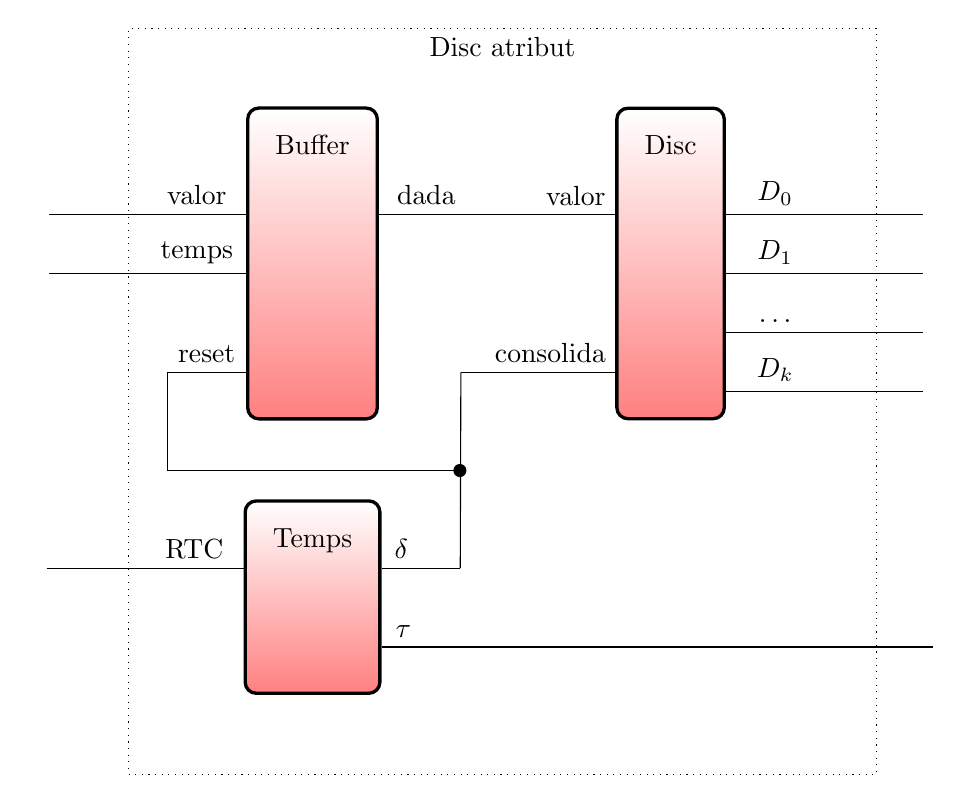
\begin{tikzpicture}
\tikzset{
    maquina/.style={rectangle,rounded corners,draw=black, 
      very thick, inner sep=1em, minimum size=3em, text centered,
      groc},
    interficie/.style={rectangle,rounded corners,draw=black, 
       inner sep=0.2em, minimum size=1em, text centered,
      verd},
    modul/.style={rectangle,rounded corners,draw=black, 
      very thick, inner sep=1em, minimum size=3em, text centered,
      roig},   
    myarrow/.style={->, >=latex', shorten >=1pt, thick},
    fletxaswitch/.style={<->, >=latex',shorten >=10pt,shorten <=10pt, thick},
    mylabel/.style={text width=7em, text centered},
    groc/.style={top color=white, bottom color=yellow!50},
    verd/.style={top color=white, bottom color=green!50},
    roig/.style={top color=white, bottom color=red!50},
  }  

  
   \node (discres) [draw, dotted, minimum width=9.5cm, text depth=9cm, rectangle] {Disc atribut};



  \node[modul,text depth=3cm,below right=1cm and 1.5cm of discres.north west] (buffer) {Buffer};  

  %entrades
  \node[above left=-1.5cm and 2.5cm of buffer.north west] (buffer_valor)   {};
  \draw[-] (buffer_valor) -- (buffer_valor-|buffer.west)
   node[near end,above]{valor};

   \node[below=0.5cm of buffer_valor] (buffer_nou)   {};
   \draw[-] (buffer_nou) -- (buffer_nou-|buffer.west)
   node[near end,above]{temps};

   \node[above left=-3.5cm and 1cm of buffer.north west] (buffer_consolida) {};
   \draw[-] (buffer_consolida) -- (buffer_consolida-|buffer.west)
   node[pos=0.5,above]{reset};

   %sortides
   \node[above right=-1.5cm and 1.5cm of buffer.north east] (buffer_dada)   {};
  \draw[-] (buffer_dada) -- (buffer_dada-|buffer.east)
   node[pos=0.6,above]{dada};





  \node[modul,right=3cm of buffer,text depth=3cm] (disc)   {Disc}; 

  % entrades
  \node[above left=-1.5cm and 2cm of disc.north west] (disc_valor)   {};
  \draw[-] (disc_valor) -- (disc_valor-|disc.west)
   node[near end,above]{valor};

  \node[above left=-3.5cm and 1.96cm of disc.north west] (disc_consolida)   {};
  \draw[-] (disc_consolida) -- (disc_consolida-|disc.west)
   node[pos=0.58,above]{consolida};

   % sortides
   \node[above right=-1.5cm and 2.5cm of disc.north east] (disc_d0)   {};
   \draw[-] (disc_d0) -- (disc_d0-|disc.east)
   node[near end,above]{$D_0$};

   \node[below=0.5cm of disc_d0] (disc_d1)   {};
  \draw[-] (disc_d1) -- (disc_d1-|disc.east)
   node[near end,above]{$D_1$};

   \node[below=0.5cm of disc_d1] (disc_d2)   {};
  \draw[-] (disc_d2) -- (disc_d2-|disc.east)
   node[near end,above]{$\dots$};

   \node[below=0.5cm of disc_d2] (disc_d3)   {};
  \draw[-] (disc_d3) -- (disc_d3-|disc.east)
   node[near end,above]{$D_k$};




  \node[modul,below=1cm of buffer,text depth=1.5cm] (temps)   {Temps}; 

  % entrades
  \node[above left=-1cm and 2.5cm of temps.north west] (temps_rtc)   {};
  \draw[-] (temps_rtc) -- (temps_rtc-|temps.west)
   node[near end,above]{RTC};

  % sortides
   \node[above right=-1cm and 1cm of temps.north east] (temps_delta)   {};
   \draw[-] (temps_delta) -- (temps_delta-|temps.east)
   node[near end,above]{$\delta$};

   \node[above right=-2cm and 7cm of temps.north east] (temps_tau)   {};
   \draw[-] (temps_tau) -- (temps_tau-|temps.east)
   node[pos=0.96,above]{$\tau$};








   %connexions
   \draw[-] (temps_delta.west) -- (disc_consolida.east); 
   
%   \node[above left=0.3cm and 1cm of temps.north west] (tau_reset)   {};
   \node[below=1cm of buffer_consolida] (tau_reset)   {};
   \draw[-*,shorten >=-2pt] (tau_reset) -- (tau_reset-|disc_consolida.east);
   \draw[-] (tau_reset.east) -- (tau_reset.east|-buffer_consolida);



\end{tikzpicture}
\caption{Esquema genèric d'un disc resolució}
\label{fig:vhdl:disc-resolucio}
\end{figure}


Condicions:
\begin{itemize}
\item Àmbit: xarxes de sensors
\item No apte per processos industrials ni llaços de control, en els
  quals cal tenir totes les dades
\item Possibilitat de validació de dades del sensor (en el buffer) i
  generar avisos de funcionament incorrecte.
\item Interfície per a consulta les dades?
\end{itemize}





Estructures alternatives:
\begin{itemize}
\item timestamps absoluts: $\delta$ creats a partir de RTC
\item timestamps relatius: $\delta$ creats a partir del clock
\item timestamps creixents: l'RTC el marca el temps de la mesura
\item Memòria estàtica en comptes de volàtil. Útil per a: a) tenir dades permanents en cas d'apagada o b) per a poder consumir menys (?)   ->  tot això no seria millor fer-ho per programa (CPU) que implementat físicament (aleshores seria més reprogramable)?
\end{itemize}





Base de dades completa, conjunt de discs resolució:
\usetikzlibrary{shapes,arrows,positioning}

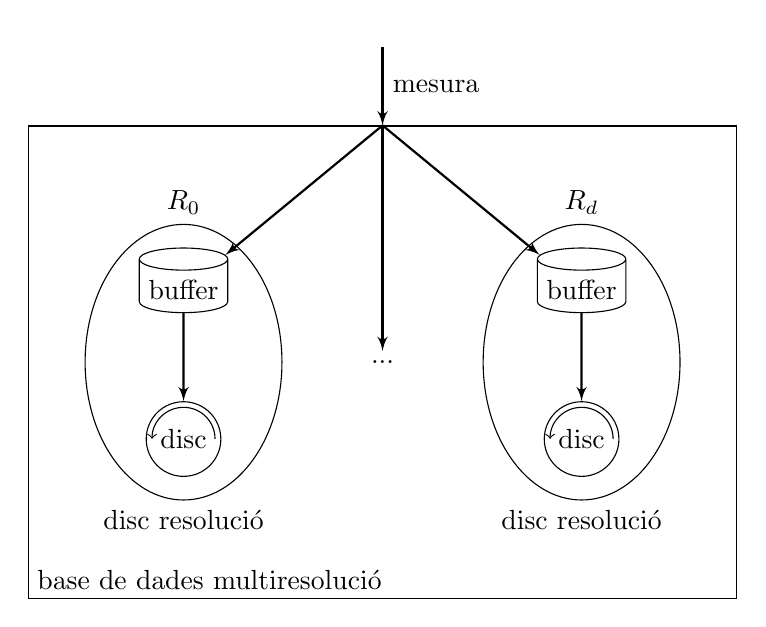
\begin{tikzpicture}
 \tikzset{
        myarrow/.style={->, >=latex',  thick},
      }
      

  \node[rectangle,draw,minimum height=6cm,minimum width=9cm] (m) {};
  \draw[shift=( m.south west)]   
  node[above right] {base de dades multiresolució};


  %discmig
  \node (m.center) (discr1) {...};

  %discr
  
  \node[ellipse,draw,minimum height=3.5cm,minimum width=2.5cm,alias=discr0] [left=of discr1] {};
  \node[above=0cm of discr0.north] {$R_0$};
  \node[below=0cm of discr0] {disc resolució};

  \node[cylinder, draw, shape border rotate=90, aspect=0.25,alias=buffer0] [below=3mm of discr0.north] {buffer};
  \node[circle, draw,alias=disc0]  [above=3mm of discr0.south] {disc} ;
  \draw [->] (disc0.center)++(.4:.4cm) arc(0:180:.4cm);
  \draw[myarrow] (buffer0.bottom) -- (disc0.north);


  %discrd

  \node[ellipse,draw,minimum height=3.5cm,minimum width=2.5cm,alias=discrd] [right=of discr1] {};
  \node[above=0cm of discrd] {$R_d$};
  \node[below=0cm of discrd] {disc resolució};

  \node[cylinder, draw, shape border rotate=90, aspect=0.25,alias=bufferd] [below=3mm of discrd.north] {buffer};
  \node[circle, draw,alias=discd]  [above=3mm of discrd.south] {disc} ;
  \draw [->] (discd.center)++(.4:.4cm) arc(0:180:.4cm);
  \draw[myarrow] (bufferd.bottom) -- (discd.north);



  %mesura 
  \node[above=1cm of m.north] (m0) {};

  \draw[myarrow] (m0) -- (m.north) 
  node[right,midway] {mesura};

  \draw[myarrow] (m.north) -- (buffer0);
  \draw[myarrow] (m.north) -- (bufferd);
  \draw[myarrow] (m.north) -- (discr1);

\end{tikzpicture}




Base de dades amb discs resolució enllaçats:

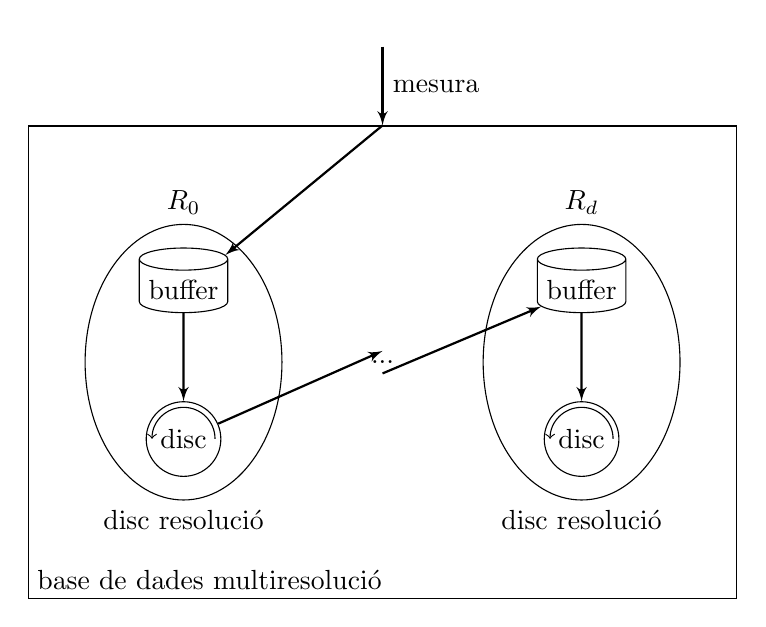
\begin{tikzpicture}
 \tikzset{
        myarrow/.style={->, >=latex',  thick},
      }
      

  \node[rectangle,draw,minimum height=6cm,minimum width=9cm] (m) {};
  \draw[shift=( m.south west)]   
  node[above right] {base de dades multiresolució};


  %discmig
  \node (m.center) (discr1) {...};

  %discr
  
  \node[ellipse,draw,minimum height=3.5cm,minimum width=2.5cm,alias=discr0] [left=of discr1] {};
  \node[above=0cm of discr0.north] {$R_0$};
  \node[below=0cm of discr0] {disc resolució};

  \node[cylinder, draw, shape border rotate=90, aspect=0.25,alias=buffer0] [below=3mm of discr0.north] {buffer};
  \node[circle, draw,alias=disc0]  [above=3mm of discr0.south] {disc} ;
  \draw [->] (disc0.center)++(.4:.4cm) arc(0:180:.4cm);
  \draw[myarrow] (buffer0.bottom) -- (disc0.north);


  %discrd

  \node[ellipse,draw,minimum height=3.5cm,minimum width=2.5cm,alias=discrd] [right=of discr1] {};
  \node[above=0cm of discrd] {$R_d$};
  \node[below=0cm of discrd] {disc resolució};

  \node[cylinder, draw, shape border rotate=90, aspect=0.25,alias=bufferd] [below=3mm of discrd.north] {buffer};
  \node[circle, draw,alias=discd]  [above=3mm of discrd.south] {disc} ;
  \draw [->] (discd.center)++(.4:.4cm) arc(0:180:.4cm);
  \draw[myarrow] (bufferd.bottom) -- (discd.north);



  %mesura 
  \node[above=1cm of m.north] (m0) {};

  \draw[myarrow] (m0) -- (m.north) 
  node[right,midway] {mesura};

  \draw[myarrow] (m.north) -- (buffer0);
  \draw[myarrow] (discr1.south) -- (bufferd);
  \draw[myarrow] (disc0) -- (discr1.north);

\end{tikzpicture}









\begin{tikzpicture}[circuit logic IEC,
  every circuit symbol/.style={
    logic gate IEC symbol color=black,
    fill=blue!20,draw=blue,very thick}]
  \matrix[column sep=7mm]
  {
    \node (i0) {0}; &
    & \\
    & \node [and gate] (a1) {}; & \\
    \node (i1) {0}; &
    & \node [or gate] (o) {};\\
    & \node [nand gate] (a2) {}; & \\
    \node (i2) {1}; &
    & \\
  };
  \draw (i0.east) -- ++(right:3mm) |- (a1.input 1);
  \draw (i1.east) -- ++(right:3mm) |- (a1.input 2);
  \draw (i1.east) -- ++(right:3mm) |- (a2.input 1);
  \draw (i2.east) -- ++(right:3mm) |- (a2.input 2);
  \draw (a1.output) -- ++(right:3mm) |- (o.input 1);
  \draw (a2.output) -- ++(right:3mm) |- (o.input 2);
  \draw (o.output) -- ++(right:3mm);
\end{tikzpicture}








\def\degr{${}^\circ$}
\begin{tikztimingtable}
  Clock 128\,MHz 0\degr    & H   12{2C} G \\ % ends with edge
  Clock 128\,MHz 90\degr   & [C] 12{2C} C \\ % starts with edge
  Clock 128\,MHz 180\degr  & C   12{2C} G \\ % ends with edge
  Clock 128\,MHz 270\degr  &     12{2C} C \\
\end{tikztimingtable}





\subsection{Possibles aplicacions}

Exemple d'aparell encastat molt petit, per exemple un aparell que
s'hagi de posar dins del cos per a mesurar la temperatura, a on hi ha
molt poc espai disponible i només permet emmagatzemar 100 dades. Es
poden desar 100 valors cada hora = 4 dies, o bé es pot aplicar una
solució de multiresolució i desa 75 valors cada hora = 2 dies i 25
valors cada dia = 25 dies. Així si no s'és a temps de recuperar les
dades en quatre dies sempre hi haurà alguna informació.

Exemple de la implementació de circuits integrats en materials molt prims i doblegables.






%%% Local Variables:
%%% TeX-master: "main"
%%% End:
